\subsection{Core --- The Model for Sequences and Choices}\label{subsec:seqcore}

This section will present the model of Sequence what the fields which have not been presented in \myref{pictogramendpoint}, are used for.

\myref{fig:sequencemodel} presents a class diagram of \texttt{Sequence} and the fields of the classes are also shown.
We present the fields of the classes \texttt{Choice} and \texttt{Sequence} as these are the only classes which were not presented in \myref{pictogramendpoint}.

\begin{figure}[h]
    \centering
    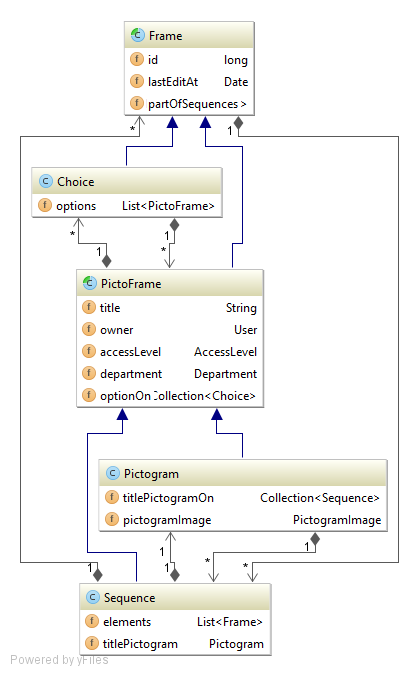
\includegraphics[width=0.5\textwidth]{figures/diagram-sequence-with-fields.png}
    \caption{Class--diagram including fields of the classes involved in Sequence}\label{fig:sequencemodel}
\end{figure}\todo{Klassediagrammet har ikke user på, selvom den har reference til sin ejer osv. skal det med ? Man kan jo se det på det fulde skema I guess ? - Søren}


\subsubsection{Sequence}
\begin{description}
	\item[elements] A list of Frames which will be shown on the \texttt{Sequence}.
	These are the Frames which a citizen have to go through on a Sequence, it is therefore important that these are in a certain order.
	\item[titlePictogram] This is the Pictogram which will be shown before beginning the \texttt{Sequence} in the app.
	This is simply a \texttt{Pictogram} formed by a \texttt{One-To-One}.
\end{description}

\subsubsection{Choice}

\begin{description}
	\item[options] Like in a \texttt{Sequence} a \texttt{Choice} needs a list of elements, but this is not a Frame it is instead a \texttt{PictoFrame} which means a \texttt{Choice} cannont have another \texttt{Choice}.
	These also need to come in the same order, as the citizens need the apps to behave the same everytime they use it, therefore if a \texttt{Choice} is made frequently the options should be places in the same spot on the view.
\end{description}

